\documentclass[12pt,a4paper,french,fleqn]{beamer}

\usepackage{tikz}

\begin{document}

\begin{frame}
    \begin{figure}
        \center
        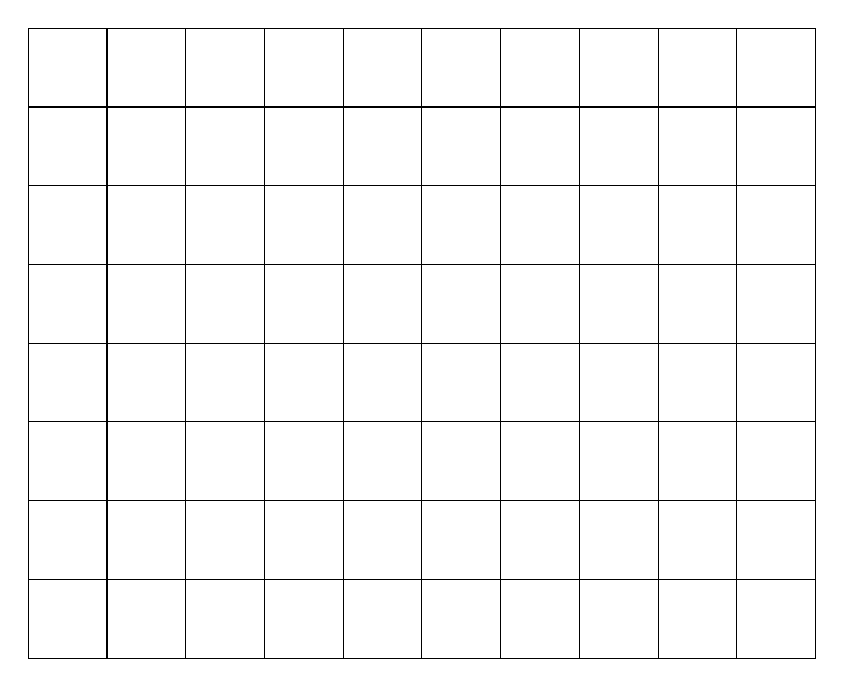
\begin{tikzpicture}
            \draw (0,0) grid (10,8);
        \end{tikzpicture}
    \end{figure}
\end{frame}

\begin{frame}
    \begin{figure}
        \center
        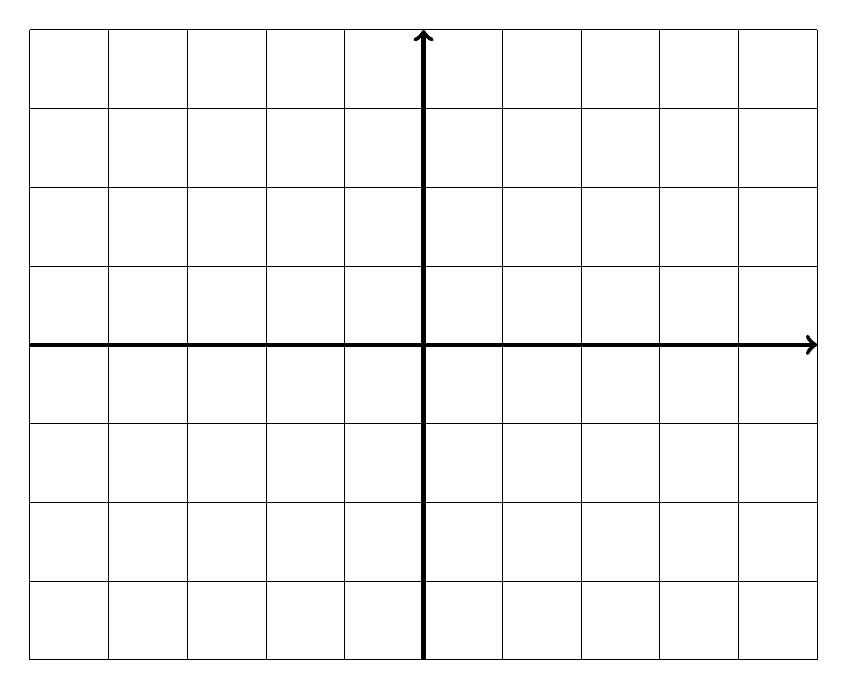
\begin{tikzpicture}
            \draw (-5,-4) grid (5,4);
            \draw [ultra thick,->] (0,-4)-- (0,4);
            \draw [ultra thick,->] (-5,0)-- (5,0);
        \end{tikzpicture}
    \end{figure}
\end{frame}

\begin{frame}
    \begin{figure}
        \center
        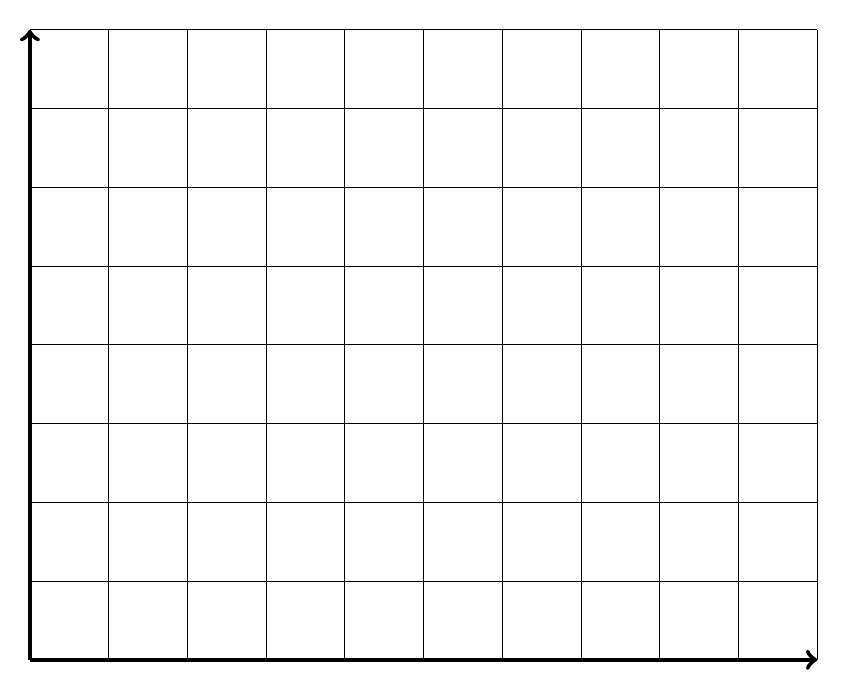
\begin{tikzpicture}
            \draw (-5,-4) grid (5,4);
            \draw [ultra thick,->] (-5,-4)-- (-5,4);
            \draw [ultra thick,->] (-5,-4)-- (5,-4);
        \end{tikzpicture}
    \end{figure}
\end{frame}


\end{document}
